\chapter{Dashboards}

Los paneles de información (en inglés \textit{dashboard}) son herramientas gráficas que nos permiten visualizar datos para convertirlos en información sin tener que realizar ningún tipo de programación.

Podríamos decir que los paneles son un interfaz gráfico previamente programado que obtiene datos de una fuente de datos (una hoja de cálculo, un fichero CSV, una base de datos,...) para posteriormente visualizarlo de una forma gráfica.

\chapter{Características}

Los paneles de información suelen contar con las siguientes características:

\begin{itemize}
    \item Son \textbf{fáciles de usar}: no es necesario ser programador para hacer uso de ellos, \textbf{siempre y cuando los datos los tengamos en un formato correcto}.
    \item Permiten hacer uso de \textbf{diferentes tipos de gráficos}: tablas, mapas para datos geolocalizados, mapas de calor, gráficos tipo tarta, mapas de barras (horizontales y verticales), ...

    \item Son \textbf{interactivos}: podemos hacer que los gráficos estén enlazados entre sí, y de esta manera al seleccionar un apartado de uno, el resto se actualizan.

    \begin{center}
        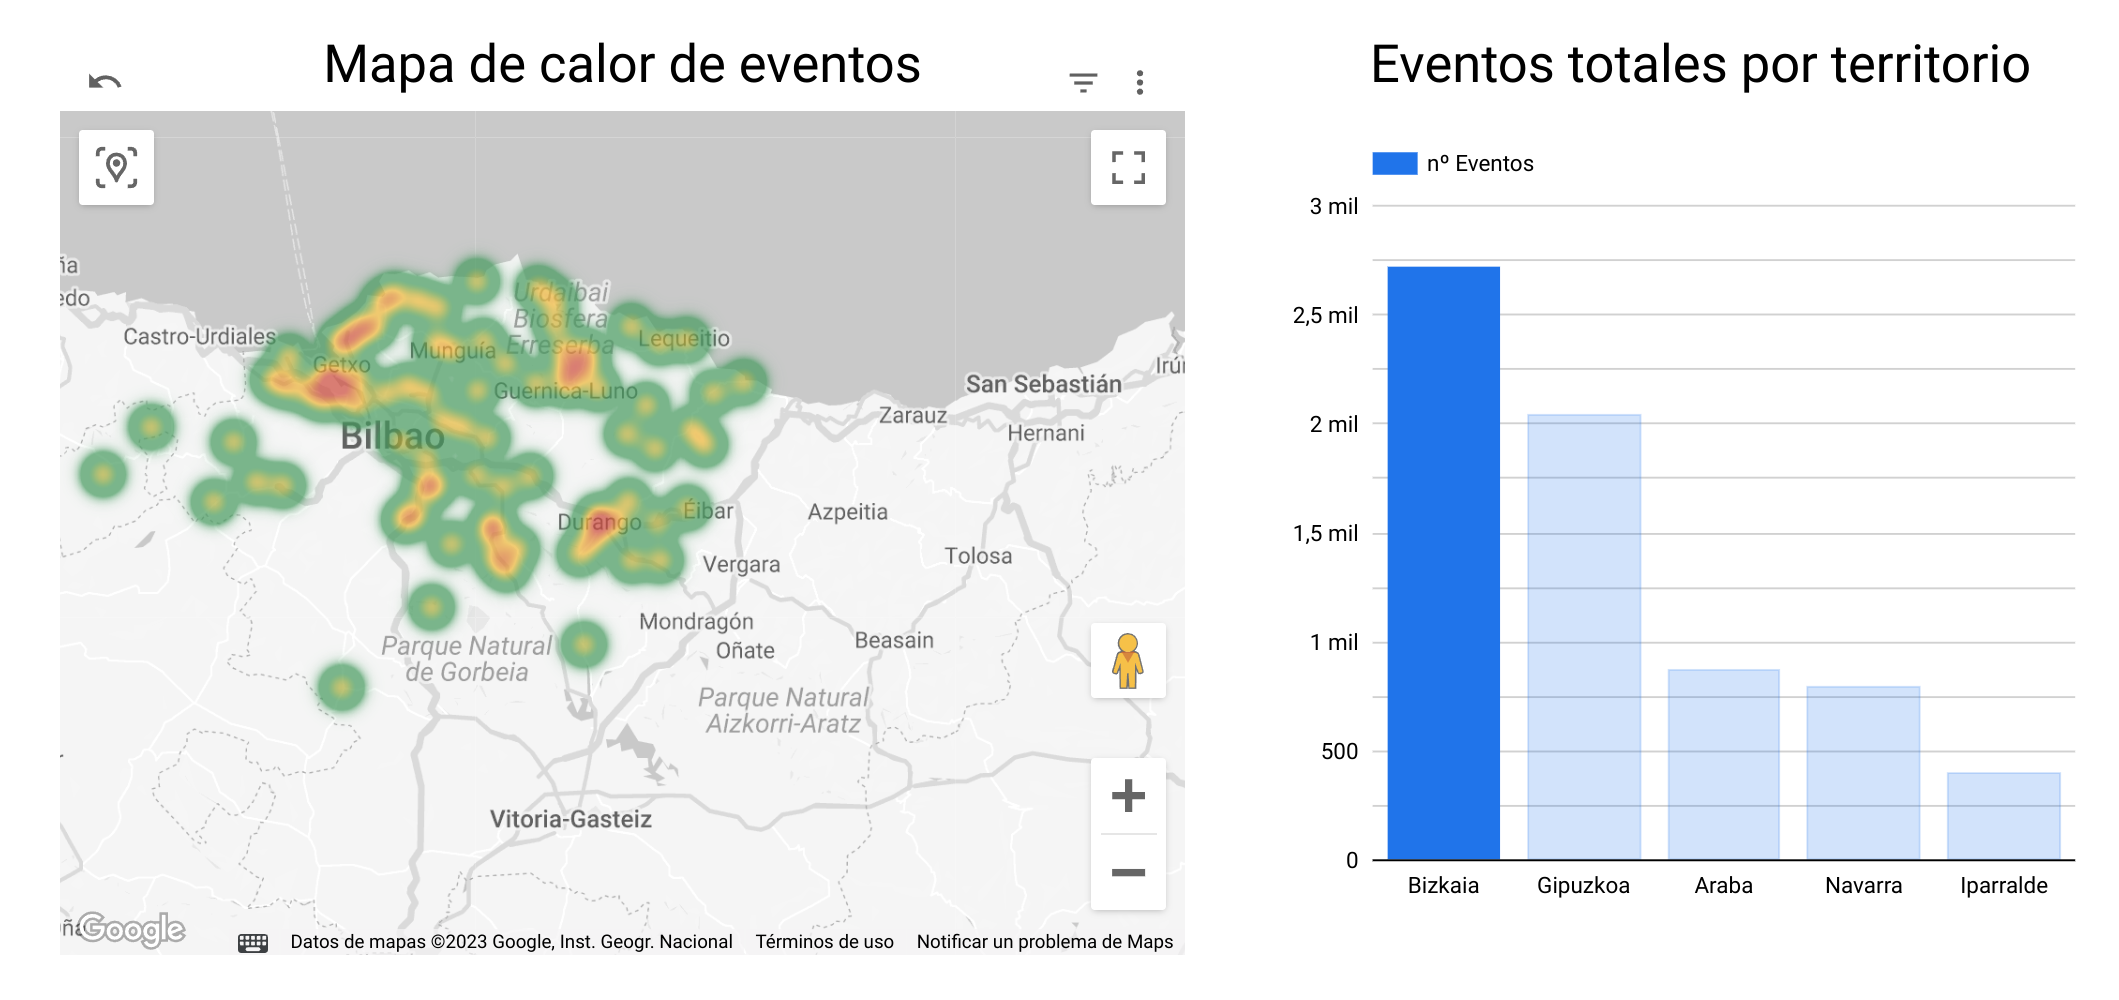
\includegraphics[frame,width=0.9\linewidth]{graficos.png}
        \captionof{figure}{Gráficos enlazados}
    \end{center}

    \item Se pueden generar \textbf{filtros} para realizar una búsqueda en los datos.

    \item Podemos \textbf{compartir} el dashboard creado o generar una presentación.

\end{itemize}


Como contrapartida, también pueden existir algunos inconvenientes a la hora de utilizarlos, que debemos de tener claros antes de utilizarlos:

\begin{itemize}
    \item Estamos \textbf{limitados a las características que ofrecen}. Por lo tanto, si nos interesa crear un gráfico distinto a los que ofrece, no vamos a poder hacerlo.

    \item Los datos deben de estar en el \textbf{formato que acepte la herramienta}. Si programamos nosotros, el formato puede ser propio, o el diccionario de datos puede estar a nuestro gusto.

    \item \textbf{Dependencia} de la herramienta. Si deciden eliminar funcionalidades, hacerla de pago, ... deberemos migrar los datos y crear de nuevo el panel.

\end{itemize}


\chapter{Entendiendo los datos}

Antes de crear un panel de información debemos tener claro los tipos de datos que tenemos, cómo están organizados (o si debemos organizarlos), en qué formato están, ... es por eso que debemos realizar un análisis previo de los mismos.

\section{Análisis de datos}

A la hora de realizar el análisis de datos, debemos tener en cuenta, al menos, las siguientes características:

\begin{itemize}
    \item \textbf{Fuente de los datos}: ¿son datos propios? ¿podemos recuperarlos en cualquier momento? ¿son fiables?

    \item \textbf{Formato de los datos}: Debemos tener en cuenta no sólo el formato del fichero en el que obtenemos los datos, si no si estos están normalizados. Por ejemplo, si los números están guardados en formato entero/real o en formato texto; si existen datos de geolocalización, si están separados o agregados; ...

    \item \textbf{Entender los datos}: Aunque pueda parecer obvio, es necesario \textbf{entender cada apartado de los datos} para posteriormente relacionarlos entre sí, y para hacer uso de ellos en el panel/gráfico.
\end{itemize}


\section{Creación del esquema de datos}
Teniendo en cuenta el punto anterior, quizá sea necesario normalizar los datos o crear un formato específico. Por lo tanto, debemos de conocer algún tipo de herramienta o de lenguaje de programación que nos permita hacerlo.

Si los datos en bruto obtenidos no cumplen las expectativas, entre las tareas que debemos realizar estarán:

\begin{itemize}
    \item \textbf{Normalizar los datos}: A cada tipo de datos convertirlo al formato que debe ser. Por ejemplo, en algunos datos de geoposición de \href{https://opendata.euskadi.eus/inicio/}{OpenData Euskadi}, hacen uso de un formato llamado \href{https://en.wikipedia.org/wiki/Universal_Transverse_Mercator_coordinate_system}{UTM}, que es necesario convertir a latitud y longitud.
    \item \textbf{Diccionario de datos}: Crear el esquema/diccionario de datos que mejor se adecúe a los datos y al sistema de panel que vayamos a utilizar.

\end{itemize}

\section{Crear el tipo de fichero}
Por útlimo, será necesario generar el tipo fichero con el formato que la herramienta necesita: json, CSV, formato excel, ...

Para ello, dependiendo del esquema de datos, podremos generar el fichero con herramientas simples (por ejemplo excel, para generar un fichero en formato CSV) o deberemos hacer uso quizá de lenguajes de programación con librerías específicas que nos faciliten la labor (por ejemplo python).

\section{Documentación del análisis}
Siempre es recomendable documentar el proceso del análisis de datos para entender en etapas sucesivas, o tiempo después, el por qué se han modificado los datos tal como se ha hecho, o la razón de hacer uso de un tipo de fichero y no otro.

La documentación también facilitará el realizar modificaciones más adelante o para poder realizar adaptaciones a nuevas herramientas. De esta manera, en principio, tendremos parte del trabajo hecho y no habrá que volver a realizarlo.

\chapter{Looker Studio como generador de paneles de información}

\href{https://lookerstudio.google.com/}{Looker Studio}, anteriormente DataStudio, es una herramienta de Google para visualizar y crear paneles informativos con datos que proporcionamos desde distintas fuentes.

Es una herramienta gratuita, fácil de usar y que permite generar distintos tipos de paneles con los datos proporcionados. Aparte, también permite crear otros tipos de visualizaciones, por lo que la comunidad aporta nuevos \href{https://lookerstudio.google.com/visualization}{paneles}.

Para poder crear los paneles, necesitaremos hacer uso de datos, que podremos importar o usar desde distintas fuentes, como por ejemplo:
\begin{itemize}
    \item Ficheros CSV (comma separated value)
    \item Hojas de cálculo de Google
    \item Bases de datos MySQL, PostgreSQL, SQL Server, ...
    \item Otros conectores creados por la comunidad
\end{itemize}

\section{Obtener datos}

En primer lugar vamos a necesitar crear una fuente de datos, donde deberemos subir los datos obtenidos. Tal como se ha dicho previamente, es necesario realizar un análisis de los mismos para posteriormente normalizarlos en caso necesario.

{
\begin{minipage}{0.3\linewidth}
    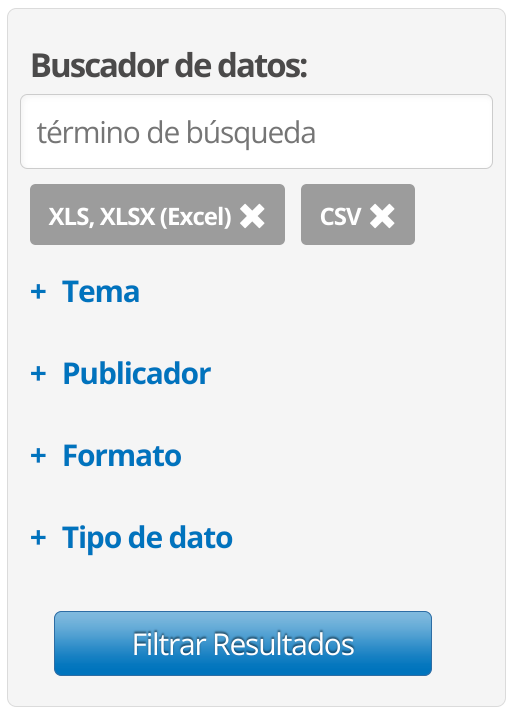
\includegraphics[width=\linewidth]{opendata.png}
    \captionof{figure}{Realizar búsqueda en \href{https://opendata.euskadi.eus/inicio/}{OpenData Euskadi}}
\end{minipage}
\hfill
\begin{minipage}{0.63\linewidth}
    \setlength{\parindent}{0em} % identation
    \setlength{\parskip}{1.2em}
    \renewcommand{\baselinestretch}{1.4}


    Para este ejemplo se va a hacer uso de una hoja de cálculo de Google con datos obtenidos de \href{https://opendata.euskadi.eus/inicio/}{OpenData Euskadi}. Buscaremos para que los datos estén en formato CSV y/o XLS de Excel, y de esta manera la conversión de los datos no resulte tan compleja.

    En caso de estar en formato \href{https://es.wikipedia.org/wiki/JSON}{JSON}, u otro, quizá deberíamos realizar una conversión previa. Aparte, de que en caso de querer realizar la manipulación de los datos, no sería tan directa.

    Tras realizar la búsqueda obtendremos un listado de resultados, en el que podremos analizar si son de nuestro interés. En algunos casos los nombres son bastante representativos. Buscaremos datos que sean de nuestro interés y que tengan datos de geolocalización.
\end{minipage}
}

Una vez descargado los datos, y generado una hoja de cálculo en Google con ellos, deberemos realizar el análisis de los datos. Entre otras cosas, deberíamos:
\begin{itemize}
    \item Renombrar la primera fila, para que cada columna esté identificada de manera correcta.
    \item Comprobar si hay datos duplicados que se puedan borrar.
    \item Eliminar columnas que no nos interesen y/o que estén vacías
    \item Comprobar si los datos geográficos están en el formato adecuado. Para ello, podremos ver si al usarlos en Google Maps hacen referencia a la localidad correspondiente.
    \begin{itemize}
        \item Los datos latitud y longitud deben estar en la misma celda y separado por una coma.
        \item En caso de estar en formato UTM, habría que convertirlos (se puede usar \href{https://yuki.github.io/utm-converter/}{este conversor}).
    \end{itemize}
\end{itemize}

Una vez realizado, deberíamos tener los datos listos para poder ser usados.

\section{Crear fuente de datos en Looker Studio}

Para poder hacer uso de los datos en los paneles de información, primero debemos agregar una “Fuente de datos”, por lo que para ello vamos a “Crear → Fuente de Datos”, y elegimos el conector específico que nos interese.

En el caso de utilizar una hoja de cálculo de Google, deberemos darle permisos para poder acceder, y elegiremos la hoja de cálculo que nos interese. También nos va a permitir seleccionar unas opciones durante la importación:

\begin{center}
    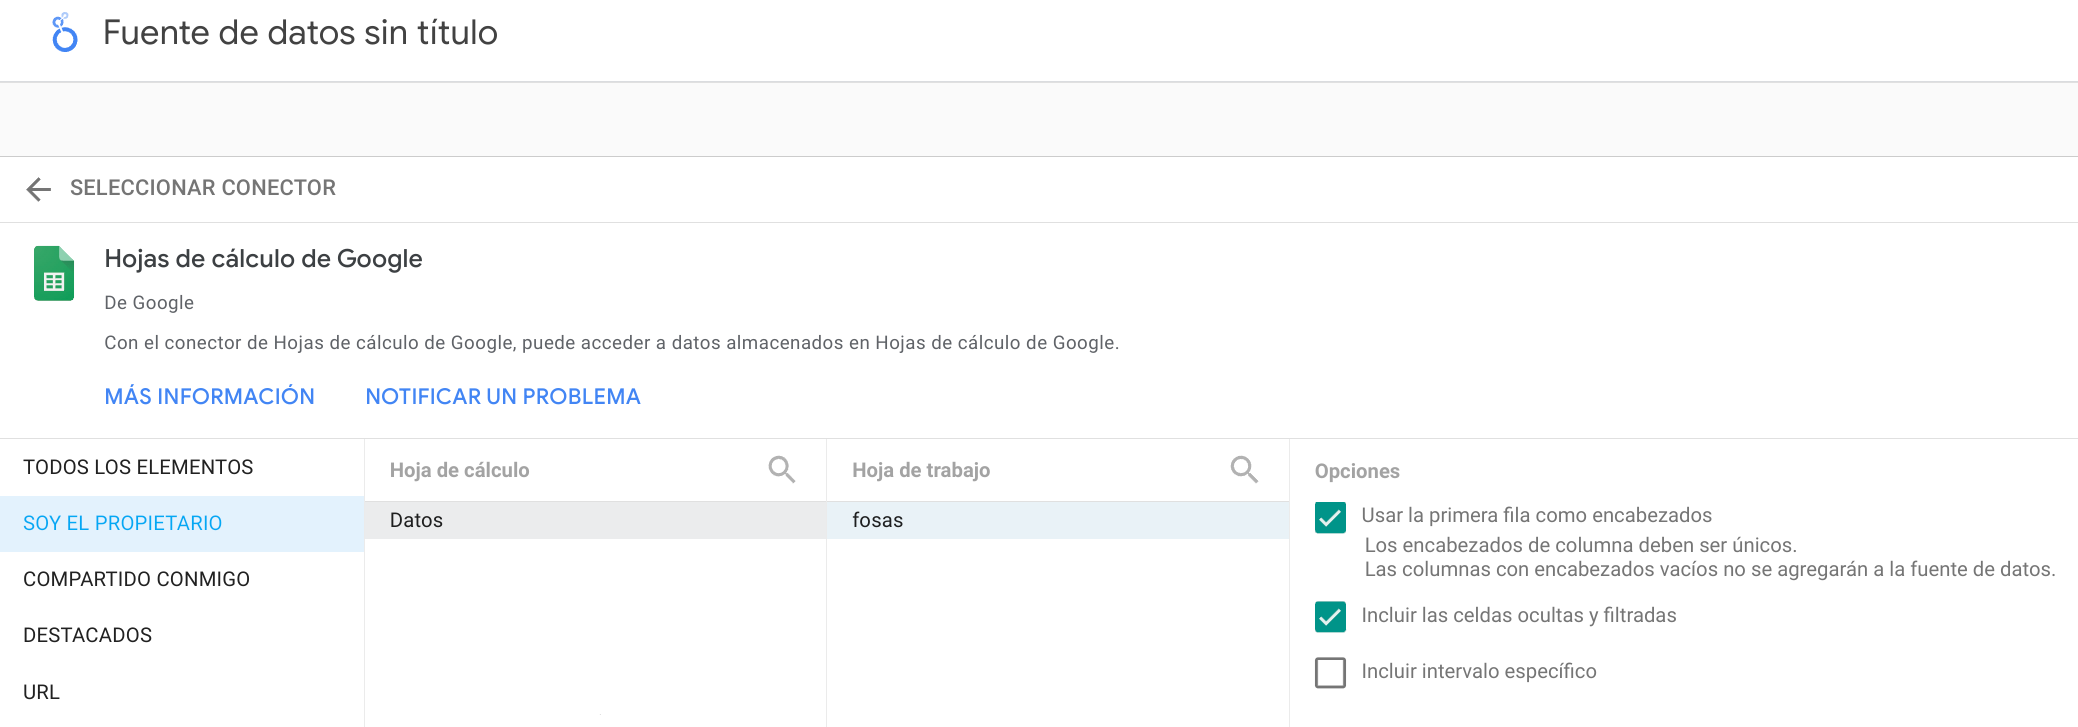
\includegraphics[frame,width=0.9\linewidth]{crear_fuente_datos.png}
    \captionof{figure}{Crear fuente de datos}
\end{center}

Tras realizar la importación, dentro de la fuente de datos deberemos identificar el tipo de fuente que es cada dato. En algunos casos Looker Studio identificará el tipo correcto, pero en otros no, como sucede con las posiciones de geolocalización.

\begin{center}
    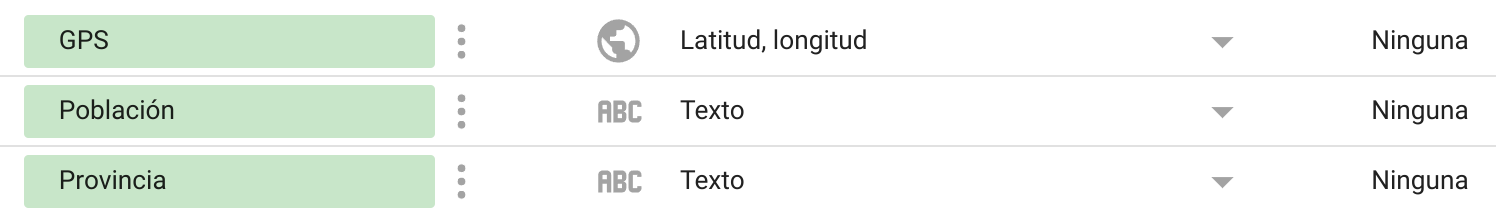
\includegraphics[frame,width=0.9\linewidth]{datos_normalizados.png}
    \captionof{figure}{Datos normalizados}
\end{center}

Una vez realizada la normalización de los datos, podemos comenzar a crear el informe.


\section{Crear informe}

Una vez terminada la normalización de los datos, es momento de comenzar a crear el informe y convertir los datos en información. Para ello, debemos pensar qué tipo de información queremos mostrar y cómo.

Looker Studio nos permite hacer uso de distintos tipos de gráficos, cada uno con sus peculiaridades y su configuración, por lo que es interesante investigar cada uno de ellos y comprobar su funcionamiento.

A continuación se explican algunos de ellos:

\begin{itemize}
    \item \textbf{Tabla}: Es la manera más sencilla de representar los datos, y tal como dice su nombre, en formato tabla, separado por filas y columnas. Podremos colocar las columnas en el orden adecuado, generar sistemas de ordenación, añadir colores a las filas pares o impares, ...

    \item \textbf{Cuadro de resultados}: Normalmente son utilizados para contabilizar el número de datos seleccionados o totales.

    \item \textbf{Gráfico de barras}: Nos muestra los datos agregados en columnas, pudiendo elegir en formato vertical, horizontal, ascendente, descendente...

    \item \textbf{Mapas}: Existen distintos tipos de mapas, que dependiendo de los datos nos permitirá visualizar datos de una manera u otra.
    \begin{itemize}
        \item \textbf{Mapa de calor}: Nos crea un mapa de calor con los datos posicionados.
        \item \textbf{Mapa de burbujas}: Geolocaliza los datos añadiendo pequeños círculos. Estos pueden ser de distintos colores identificando algún aspecto destacable de los datos.
    \end{itemize}
\end{itemize}

En el siguiente \href{https://lookerstudio.google.com/reporting/a08f1776-4f54-4421-9a3e-69f2f4130b80/page/GaKdD}{enlace} se puede ver los aspectos más básicos de un informe.